\chapter{Introduction}
\label{sec:Introduction}

\paragraph{}
A distinct problem arising from attempting to study the exact state of sea ice is that there is limited data available. Data pertaining to sea ice is widely distributed, not correlated, or limited in scope such that it's difficult to draw inferences from. Naturally, the immediate approach to this thesis will first require research into available data sources before conducting any exploration. This exploration will reveal which sources should be targeted for the remainder of the thesis.

\indent After reviewing the preliminary research, this paper will move forward to a more targeted effort in obtaining and analyzing data to develop a machine learning model that can be used to predict ice thickness from said remote sensing methods. Chapter 2 will describe the process of obtaining the selected data, and Chapter 3 will discuss the methodology of developing the model.
\par

\section{Preliminary Research}
Preliminary research into the availability of ice thickness data yields three notable organizations which may act as sources of data. These three organizations are the National Snow and Ice Data Center (NSIDC), the National Aeronautics and Space Administration (NASA), and the European Space Agency (ESA). Although all organizations offer large amounts of data, they differ in approach. The NSIDC acts as a historic repository, accumulating previous studies into a single location for easy access. NASA offers a similar service, but additionally allows researchers the opportunity to query information from any of their active orbiting satellites. The ESA, like NASA, offers near real-time satellite data but also offers to sponsor data from external companies with the completion of a project proposal.

\subsection*{NSIDC}
Here is where the NSIDC links and data retrieval should be discussed. Limitations of the data or other notes about it's composition should be included according to the details in the abstract saved on file. Preliminary exploration will be where the figures will be uploaded (Or maybe we show one figure showing all of the points, and the exploration will be for the single instance?)

\subsection*{ESA}
Here is where you discuss the ESA's copernicus portal, finding the ICEYE company, looking through the proposal process, seeing superior SAR resolution from this private company than NASA's sentinel-2

\subsection*{NASA}
Here is where you should include sources to the ATL10 Data Specification pdf, and the associated CryoSat data specs. It should also be included where these links came from. It also should be included where, if applicable, specific data downloads were from. It should include the process of querying for data, which portals are made accessible, and how flexible they are. Do not forget to mention that they made an IceSat-2 mobile application for iOS. \cite{ICESat-2-ATL10-Product}

Include how NASA's Sentinel-2 delivers SAR imaging, but at 50m resolution. This is a modality that can be used for a CNN but the resolution is not meaningfully compatible with any source of ground truth we have. Thus, searching for alternatives led to the European Space Agency and its sponsorship for ICEYE's 1m resolution imaging.

Somewhere you should discuss IceSat-2 and its laser altimetry. ESPECIALLY that it's 17m footprint offers precision at a given location, 

\section {Preliminary Exploration}
After researching the available data sources across these 3 agencies, the NSIDC's In-Situ dataset offered the greatest possibility of learning direct trends of sea ice. However, NASA's IceSat-2's predictable orbit combined with the possibility of obtaining ICEYE's high resolution SAR imaging, suggested that a temporally and spatially coincident dataset could be obtained. This intersection of remote sensed imagery with precise remotely sensed freeboard measurements, is conducive for a convolutional neural network applying IceSat-2's accuracy onto the expansiveness of SAR imaging. This model would be more dynamic in nature than the static accumulation of In-situ data, and would give more insight into the changing state of sea-ice. \cite{In-Situ-Dataset}

Importantly, it's important to recognize that laser altimetry is purely restricted to measuring Earth's surface - meaning the returned measurements are innately incapable of measuring sea-ice thickness, especially in the presence of snow on the surface. (Add source and put it in bibliography)
\begin{figure}[htb]
	\centering
	\subfigure{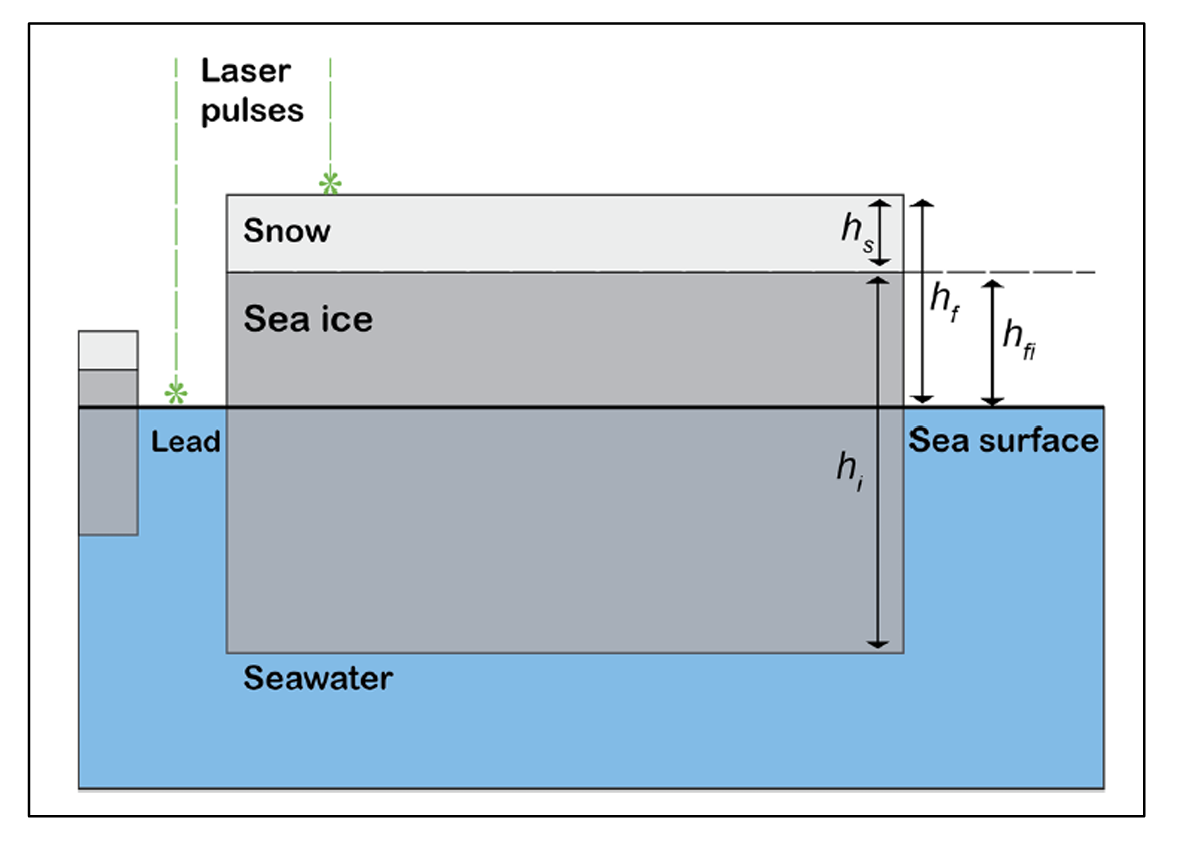
\includegraphics[width=.8\textwidth]{../research-resources/ice-sat-2/hydro-static-equillibrium.png}} 
	\caption{Laser Altimetry on a buoyant surface} \cite{ICESat-2-L4-Product}
	\label{fig:hydro-static-diagram}
\end{figure}

NASA's ICESat-2 L4 Along-Track Sea Ice Thickness highlights this problem, and addresses it using the assumption of hydro-static equilibrium. This equation, expressed as follows, uses the densities of water, sea-ice and snow, alongside the height of the snow to calculate the correlated thickness of the sea ice.

\begin{equation*}
	\rho_i
	\rho_w
	\rho_s
\end{equation*}

% Data of interest were the IceSat-2 ATL10 product and the NSIDC In-situ Dataset, selected for their combination of breadth and accuracy. Furthermore, the European Space Agency's requirements for sponsored data need to be explored to pursue the higher resolution SAR imagery hoped for. The in-situ measurements will provide an invaluable source of ground truth while the ATL10 product will drastically expand the flexibility and accessibility of sea ice freeboard data moving forward.

\subsection*{NSIDC}
\paragraph*{}
The "On-Ice Arctic Sea Ice Thickness Measurements by Auger, Core, and Electromagnetic Induction, from the Late 1800s Onward, Version 2" contains 69,750 rows of data, spanning 5 categorized regions; the Arctic Ocean, the Beaufort Sea, Greenland Coast, Prudhoe Bay, and Russian Coast. Filtering down to the Beaufort Sea region, a region of interest, yields 23 separate studies ranging between 1958 and 2016.
\par
%%% Modify which figures you're showing and in what order. It's not apparent what direction you're trying to go from here if you leave all 3 together like this.
\begin{figure}[htb]
	\centering
	\subfigure{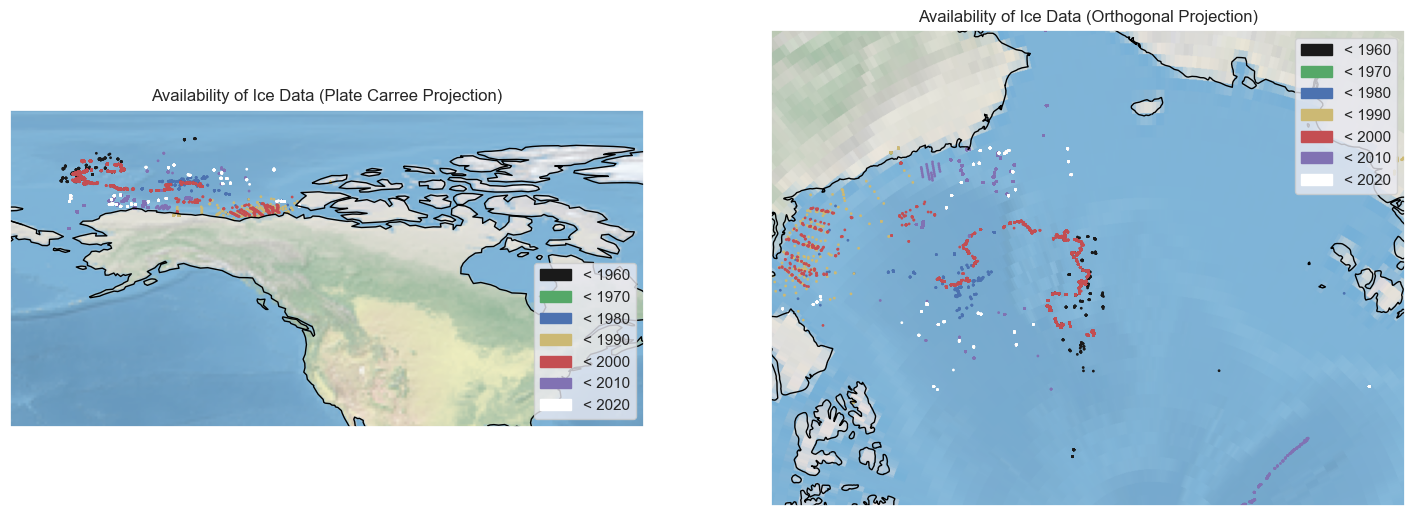
\includegraphics[width=0.8\textwidth]{../research-resources/in-situ/Plotted-Tracks.png}} 
	\subfigure{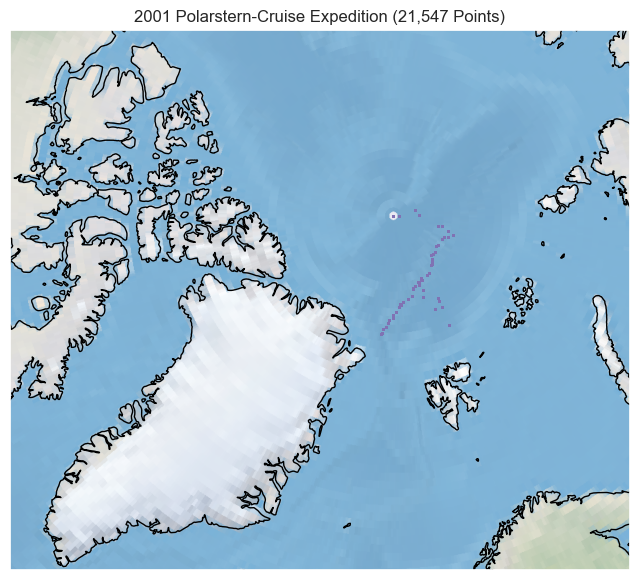
\includegraphics[width=0.5\textwidth]{../research-resources/in-situ/region-of-interest.png}} 
	\caption{In-Situ Data Availability}
	\label{fig:foobar}
\end{figure}


\paragraph*{}
For a simple analysis, the largest single dataset was chosen to conduct a simple test on the distribution of sea ice thickness. This distribution if normal will reasonably allow for future conducting of statistical tests, and if not normal will give insight as to what a reasonable assumption of ice thickness distribution should be. The largest dataset consists of 21,547 distinct points sourced from direct auger measurements and indirect electromagnetically sensed methods. Given that the majority of the data comes from the remote sensed method, it was validated by plotting the sensed values against the auger values where applicable and seeing how correlated they were. The results of a linear regression test yielded a relationship of 0.92x + 0.18, with an adjusted R\^2 value of 0.866 and a P Value of 2.31 * 10\^-202. The adjusted R\^2 value and low P value demonstrate there is a high correlation between these variables, and our model captures a significant portion of the variance. The 0 line is plotted as a way to visualize how the residuals are symmetrically clustered around 0.
\par

\begin{figure}[htb]
	\centering
	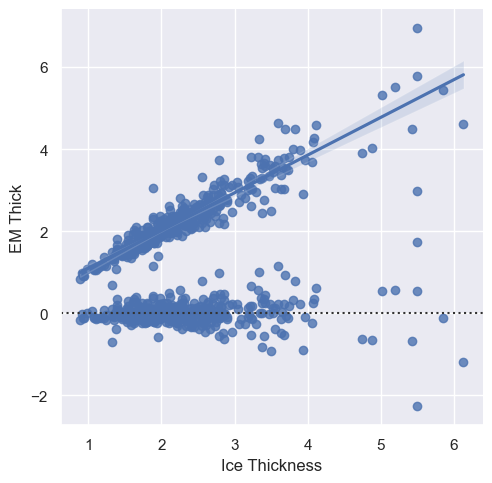
\includegraphics[width=.6\linewidth]{../research-resources/in-situ/auger-vs-em-thickness.png}
	\caption{Electromagnetic vs Auger Sourced Relationship}
	\label{fig:aug-vs-em}
\end{figure}

\paragraph*{}
After accepting the validity of the electromagnetically sensed data, the points were plotted to visualize the strip of ice that was measured. Given that these data points were taken in a single linear track, the line graph shows a cross-sectional profile of ice in that axis. The distribution reveals a slight tail on the left side of the curve, and a hypothesis test confirms that the distribution is not normal. Moving forward, it is reasonable to believe that ice distribution is not normal, and over a large enough sample there is expected to be a slight tail on either end.
\par
\begin{figure}[htb]
	\centering
	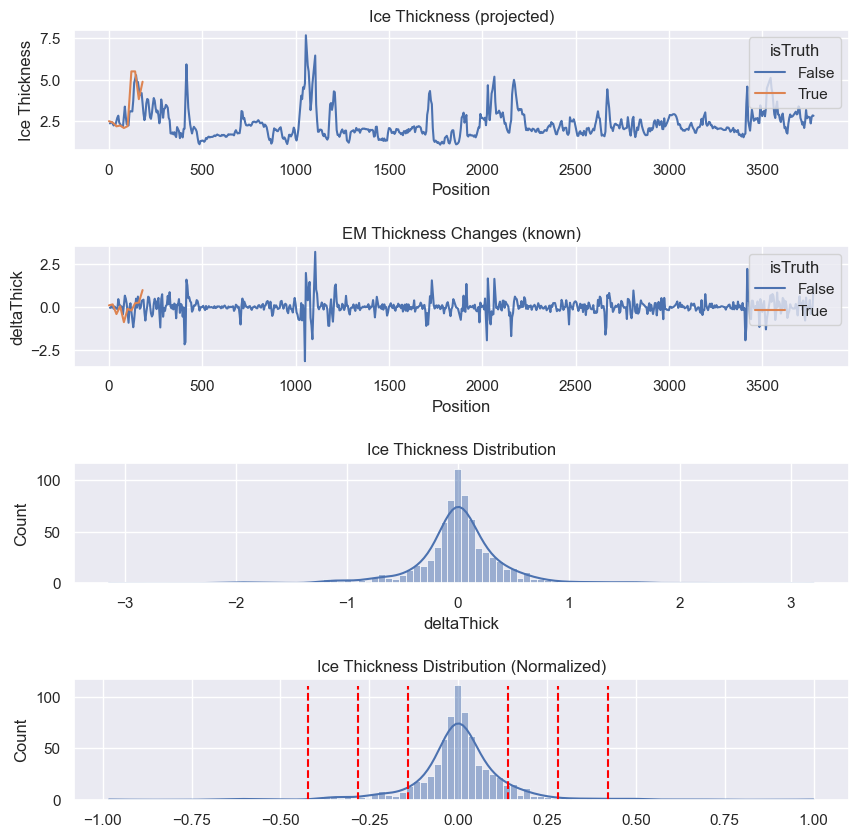
\includegraphics[width=\linewidth]{../research-resources/in-situ/track-graphs-p-test.png}
	\caption{In-Situ Ice Thickness Distribution}
	\label{fig:p-test-aug}
\end{figure}

\subsection*{NASA}
A single delivery of IceSat-2's ATL10 data product yields a '.h5' file, incompatible with traditional spreadsheets. To access IceSat-2 data in a meaningful way involved developing a script to extract relevant information according to the types enumerated in the data product specification. Columns of interest include the latitude, longitude, time, and calculated freeboard height for each of the three beam pairs.
// Consider adding perl and dynamically adding sample rows from the extracted .h5 file. This will give the reader context as to what's being gathered /


\subsection*{ESA}
Filling out the proposal for ICEYE sponsored data. (eg: See Appendix A or something)